\documentclass[11pt, a4paper]{article}
\usepackage[portuguese]{babel}
\usepackage[margin=1in]{geometry}
\usepackage{amsmath}
\pagenumbering{gobble}
\usepackage{listings}
\usepackage{graphicx}
\usepackage{wrapfig}

\graphicspath{ {./images/} }


\begin{document}
Objetivo do curso: compreensão básica de modelos de aprendizado de máquina.

\section{O que é Machine Learning?}
É uma área relativamente antiga que é estudada há várias décadas. O que chamou atenção recentemente foram as boas performances em algumas tarefas de grande interesse. Entre elas, a análise de imagens.

\textbf{Convolutional Neural Network} foi usado em escala pela primeira vez em 2012, o que mostrou sua performance. Desde lá, ela apenas melhorou. O \textbf{Deep Learning} está passando a performance humana em alguns casos na análise de imagens.

Outra área que o \textbf{Machine Learning} foram os jogos. As maquinas conseguem entender e performar melhor que um humano nos jogos. Por exemplo, um dos melhores jogadores de \textit{Go} perdeu para um humano.\\

Como realmente funciona? Basicamente, nós vamos ensinar uma máquina a aprender. Damos exemplos para ela (amostras de dados), e o que gostaríamos que ela concluísse com os dados.

\begin{figure}[h]
\centering
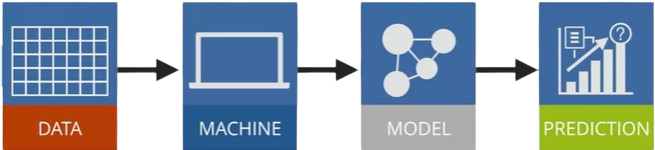
\includegraphics[scale=0.5]{linear-view}
\caption{Ordem das ações de Machine Learning.}
\end{figure}

Para treinar, damos vários exemplos nesse formato: esse conjunto de dados $x_1$ resulta nesse $y_1$, um outro conjunto $x_2$ em $y_2$ e assim por diante.

Para cada $x_i$ que ele receber, deve retornar o respectivo $y_i$; Porém, se passarmos um conjunto que não foi contemplado, ele deve ser capaz de prever qual será o resultado.

Queremos que ele aprenda os parâmtros do modelo matemático e predizir o $y_i$ dado o $x_i$.

\begin{figure}[h]
\centering
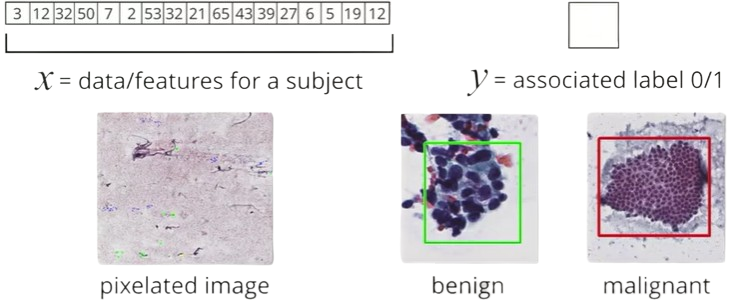
\includegraphics[scale=0.5]{exemplo-ml}
\caption{Exemplo de Machine Learning para identificar tumores benignos e malignos.}
\end{figure}

\subsection{Regressão Lógica}

Queremos um training set que consiga aprender um modelo e consegue prever o resultado dado um conjunto de dados.

Para fazer o \textit{learning} temos um algorítimo que é feito com vários parâmetros e \textit{learning} significa que gostaríamos de inferir quais parâmetros desse modelo são consistentes com nossos dados de treinamento.

Vamos considerar um dos algorítmos mais básicos: \textbf{Logistic Regression}

O objetivo do \textbf{Machine Learning} é que, dado $N$ exemplos, data $x$ e outcome $y$, gostaríamos de construir modelo preditivo que é capaz de prever $y$ dado $x$.\\

\begin{figure}[h]
\centering
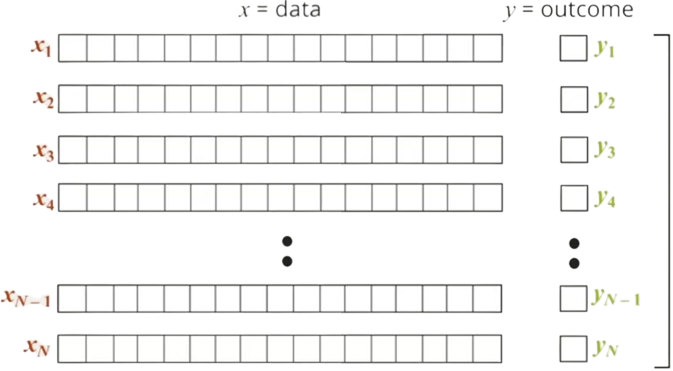
\includegraphics[scale=0.5]{exemplo-logistic-regression}
\caption{Exemplo Logistic Regression.}
\end{figure}

\textbf{Linear Predictive Model}: $X_{i1}$ é o primeiro componente do vetor $X$, $X_{i2}$ o segundo e assim por diante até $X_{iM}$.

Vamos multiplicar cada componente do vetor $X$ por um parâmtro e somamos um bias:
$$(b_1 \times x_{i1}) + (b_2 \times x_{i2}) + \dots + (b_M \times x_{iM}) + b_0 $$

Isso é um mapeamento dos dados $X_i$ para um número $Z_i$.

\begin{figure}[h]
\centering
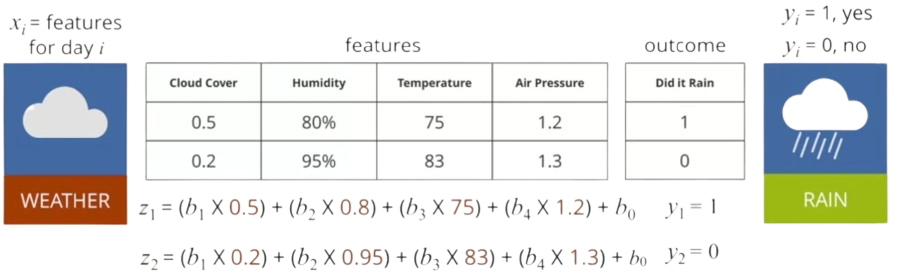
\includegraphics[scale=0.5]{exemplo-chuva}
\caption{Conjunto de dados exemplo para predizir a chuva.}
\end{figure}

Muitas vezes é melhor dar uma chance se vai chover ou não em um dia do que afirmar algo. Para fazer isso, usamos uma \textbf{Logistic Function} notado por $\sigma$:
$$ p(y_i = 1 | x_i) = \sigma (z_i) $$
$z_i$: multiplicação dos parâmetros dos dados $X$ com os parâmtros $b_1, b_2$ até $b_M$.


\begin{figure}[h]
\centering
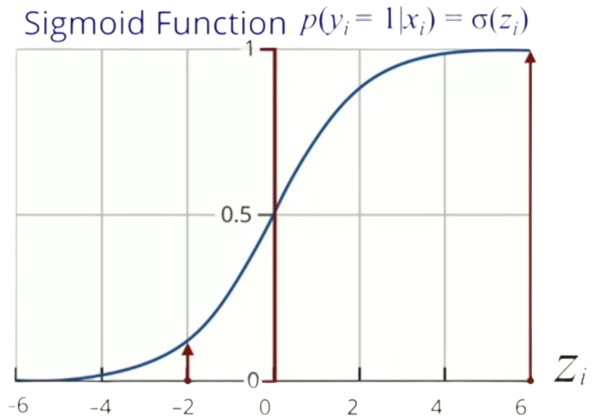
\includegraphics[scale=0.4]{sigmoid_function}
\caption{
\centering
\textbf{Sigmoid Function} é uma maneira de converter previsões para uma perspectiva probabilística.}
\end{figure}


Essa função, a \textbf{Sigmoid Function} $p(y_i = 1 | x_i) = \sigma(z_i)$, sempre está entre 0 e 1. Quando $z_i$ é grande, como 5 ou 6, a função converte ele para um número perto de 1. Quando é pequeno, -1, -2, -4, converte para perto de 0.

Os parâmetros $b$ dizem o quão importante as variáveis são para a predição.

É um modelo bem simples; é apenas uma combinação linear de multiplicação das variáveis observados pelos parâmetros associados, somando-os, mapenado eles para uma variável $z_i$ e, então, executando-os por meio de uma função Sigmoid Function.


O coração do machine learning é: temos um modelo paramétrico que é caracterizado por um conjunto de parâmetros que queremos aprender. A maneira em que fazemos o aprendizado é ter um conjunto de dados e, para esses dados, temos parâmetros $X$ e resultado $Y$. Gostaríamos de aprender os parâmetros do nosso modelo de tal forma que as predições do modelo sejam consistentes com os dados do treinamento.

O que queremos dizer com \textit{Learning} é inferir os parâmetros $B_0$ até $B_M$ que nos forneçam saídas de mapeamento de $X$ para $Y$ consistente com os dados.

Os conceitos básicos da \textbf{Logistic Regression} são bastante usados em Deep Learning.

\textbf{Logistic Regression} é um processo de modelar uma probabilidade discreta de um resultado dado os inputs. O mais comum é um binário, sim ou não.


\subsection{Interpretação da Logistic Regression}

É um dos conceitos mais simples de Machine Learning.

Exemplo para análise de escrita humana.
Dada uma foto de uma letra, queremos que a máquina diga que número que é.
\begin{figure}[h]
\centering
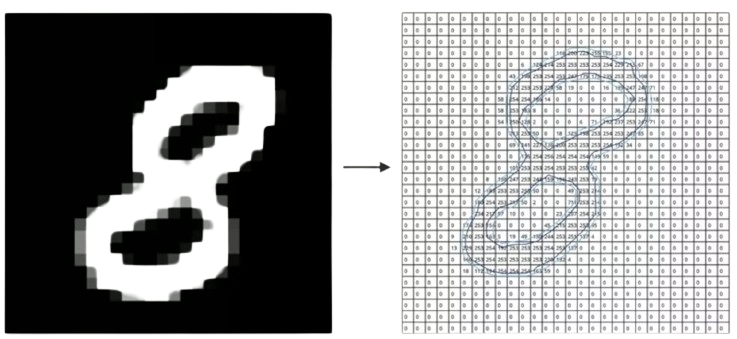
\includegraphics[scale=0.3]{8-traduzido}
\caption{8 analisado pixel a pixel.}
\end{figure}

Transformamos a imagem em uma matriz de pixels, onde cada um deles possue um peso em um espaço. Pegamos esses pixels e eles são o vetor $X$ que foi conversado anteriormente.

Primeiramente, vamos considerar o problema onde os números só podem ser 1s ou 0s para encaixar na Logistic Regression.

Os dados de treinamento são as imagens e o que representam. Seus pixels serão o vetor $X$.
Vamos ponderar os pixels multiplicando pelos parâmetros $b_1$ até $b_M$, somamos, conseguimos $Z$, passamos esse valor pela \textbf{Sigmoid Function} e conseguimos um numero entre $0$ e $1$, que diz a probabilidade de ele ser $0$ ou $1$.

\begin{center}
O que queremos dizer com \textit{learning} é inferir o conjunto de parâmetros $b_0$ a $b_M$.
\end{center}


Esse somatório matemático pode ser representado da seguinte maneira:
\[ \sum_{m=1}^{M} x_{im} \times b_m \]
\[ x_i \odot b \]
Que significa o produto interno entre $x_i$ e $b$.

Portanto, temos o valor de nosso $z_i$ dado por:

\[ z_1 = b_0 + x_i \odot b \]

Os parâmetros do modelo b são como um filtro para os dados.

\begin{figure}[h]
\centering
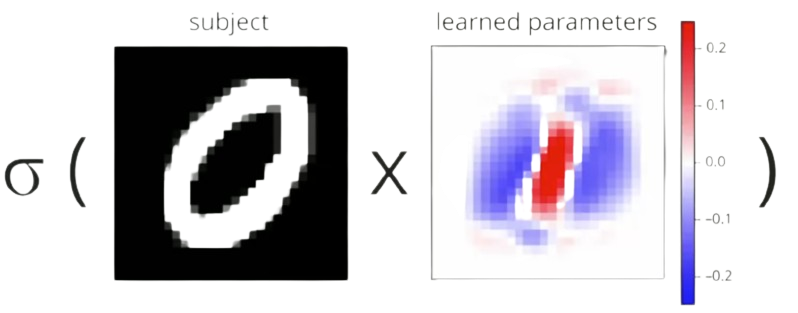
\includegraphics[scale=0.3]{filtro-sigmound}
\caption{À esquerda, o que foi recebido. À direita, o filtro que será aplicado.}
\end{figure}


\begin{figure}[h]
\centering
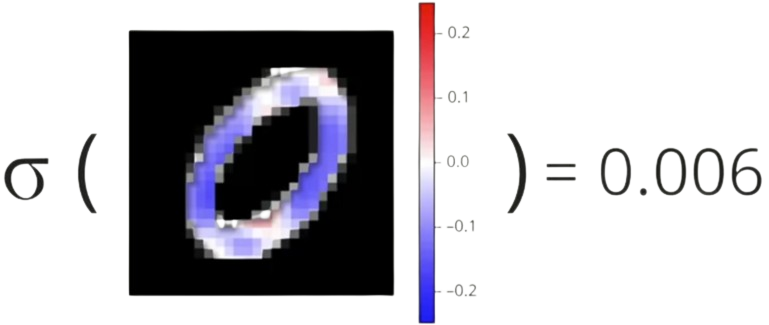
\includegraphics[scale=0.3]{resultado}
\caption{\centering Resultado do filtro; como há mais partes em azul (negativas) o produto interno $x_i \odot b$ resulta em um valor bem próximo de 0.}
\end{figure}

Esse modelo será usado como base para outros mais complexas como o Deep Learning.

\subsection{Motivação para Multilayer Perception}

Em \textbf{Logistic Regression}, nós possuíamos dados $X_i$, então fazemos um produto interno $x_i \odot b$, que chamamos de filtro, e ele é somado com $b_0$ (bias) para conseguir $z_i$. Então a \textbf{Zigmoid Function} converte esse número em uma probabilidade.

Qual é o problema com esse modelo?

Um ótimo modelo quando há diferença entre uma classe 0 e 1, que podem ser separados por uma linha. Ele está resolvendo um problema binário.

\begin{figure}[h]
\centering
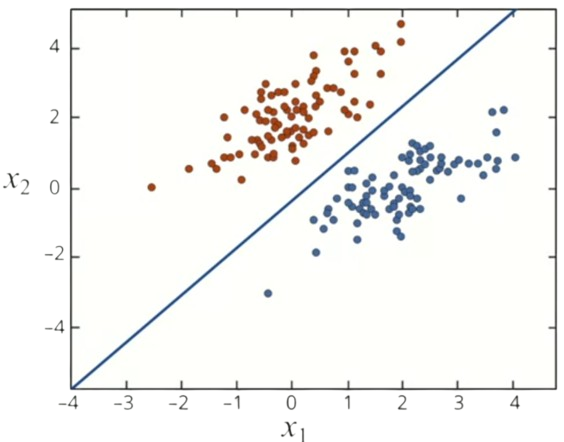
\includegraphics[scale=0.3]{bom-para-logistic-regression}
\caption{Situação em que é bom usar Logistic Regression.}
\end{figure}

Problemas as classes 1 e 0 não podem ser separados por uma linha não podem ser resolvidos pelo modelo em questão.

\begin{figure}[h]
\centering
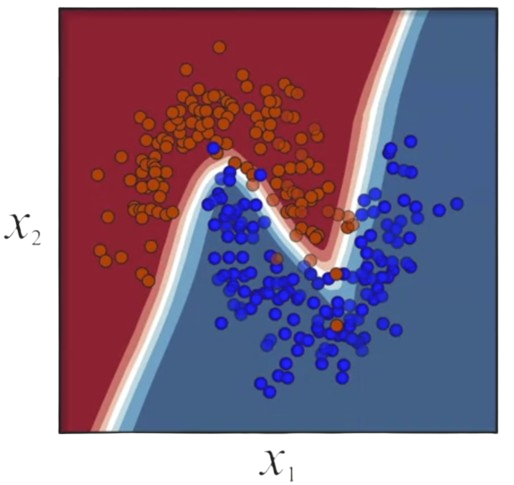
\includegraphics[scale=0.3]{ruim-para-logistic-regression}
\caption{Situação em que é ruim usar Logistic Regression.}
\end{figure}

\textbf{Logistic Regression} somente é efetivo quando um classificador linear pode ser facilmente distinguido entre classes 1 e 0.


O \textbf{Multilayer Perception} é uma extensão do \textbf{Logistic Regression} que pode ser usado para esses problemas mais complexos.

\pagebreak

\section{Conceitos Python Importantes}

\begin{lstlisting}[language=Python, caption=NumPy]
import numpy as np

x = np.array([2, 4, 6]) # create a rank 1 array
A = np.array([[1, 3, 5], [2, 4, 6]]) # create a rank 2 array
B = np.array([[1, 2, 3], [4, 5, 6]])

# Indexing/Slicing examples
print(A[0, :]) # index the first "row" and all columns
print(A[1, 2]) # index the second row, third column entry
print(A[:, 1]) # index entire second column

# Arithmetic Examples
C = A * 2 # multiplies every elemnt of A by two
D = A * B # elementwise multiplication rather than matrix multiplication
E = np.transpose(B)
F = np.matmul(A, E) # performs matrix multiplication 
# -- could also use np.dot()
G = np.matmul(A, x) # performs matrix-vector multiplication 
# -- again could also use np.dot()

# Broadcasting Examples
H = A * x # "broadcasts" x for element-wise 
# multiplication with the rows of A
print(H)
J = B + x # broadcasts for addition, again across rows
print(J)

X = np.array([[3, 9, 4], [10, 2, 7], [5, 11, 8]])
all_max = np.max(X) 
# gets the maximum value of matrix X
column_max = np.max(X, axis=0) 
# gets the maximum in each column -- returns a rank-1 array [10, 11, 8]
row_max = np.max(X, axis=1) 
# gets the maximum in each row -- returns a rank-1 array [9, 10, 11]

# In addition to max, can similarly do min. Numpy also has argmax 
to return indices of maximal values
column_argmax = np.argmax(X, axis=0) # note that the "index" here is 
# actually the row the maximum occurs for each column

total_sum = np.sum(X)
column_sum = np.sum(X, axis=0)
row_sum = np.sum(X, axis=1)

X = np.arange(16) # makes a rank-1 array of integers from 0 to 15
X_square = np.reshape(X, (4, 4)) # reshape X into a 4 x 4 matrix
X_rank_3 = np.reshape(X, (2, 2, 4)) 
# reshape X to be 2 x 2 x 4 --a rank-3 array
# consider as two rank-2 arrays with 2 rows and 4 columns

\end{lstlisting}

\begin{lstlisting}[language=Python, caption=MatPlotLib.PyPlot]
import numpy as np
import matplotlib.pyplot as plt

# We'll start with a parabola
# Compute the parabola's x and y coordinates
x = np.arange(-5, 5, 0.1)
y = np.square(x)

# Use matplotlib for the plot
plt.plot(x, y, 'b') # specify the color blue for the line
plt.xlabel('X-Axis Values')
plt.ylabel('Y-Axis Values')
plt.title('First Plot: A Parabola')
plt.show() # required to actually display the plot
\end{lstlisting}

Another Matplotlib function you'll encounter is *imshow* which is used to display images. Recall that an image may be considered as an array, with array elements indicating image pixel values. As a simple example, here is the identity matrix:


\begin{lstlisting}[language=Python]

import numpy as np
import matplotlib.pyplot as plt

X = np.identity(10)
identity_matrix_image = plt.imshow(X, cmap="Greys_r")
plt.show()

# Now plot a random matrix, with a different colormap
A = np.random.randn(10, 10)
random_matrix_image = plt.imshow(A)
plt.show()
\end{lstlisting}

\pagebreak
\section{Multilayer Perceptron}

É uma extensão direta da \textbf{Logistic Regression}. Ao invés de fazer ela 1 vez, faremos ela $k$ vezes.

\begin{figure}[h]
\centering
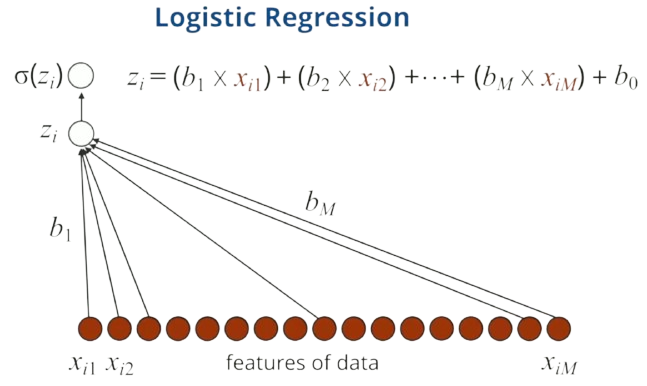
\includegraphics[scale=0.3]{1stMTP}
\caption{Logistic Regression.}
\end{figure}

Então, mapearemos nosso vetor $X$ para um vetor de $k$ dimensões chamado de \textbf{K Latent Processes/Features}, é chamado de latente porque são representações de coisas que não podemos, a principio, observar. Depois, esses $k$ recursos são enviados por um modelo de \textbf{Logistic Regression} para, no final, gerar uma probabilidade binária para a classificação dos dados.

Os $x_{iM}$ dados que possuímos primeiramente serão mapeados para $z_{i1}$ até $z_{ik}$ processos latentes, para então cada um ser transformado em probabilidades (um vetor de $k$ dimensões) que, por fim, produz um resultado: a probabilidade e que os dados correspondam à classe $y = 1$.

\begin{figure}[h]
\centering
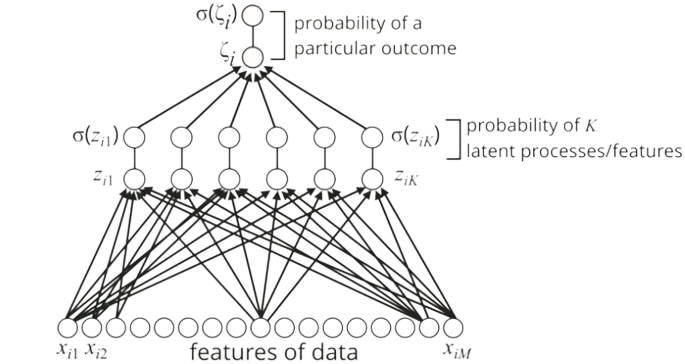
\includegraphics[scale=0.3]{2ndMTP}
\caption{Logistic Regression.}
\end{figure}

\begin{center}
Deve ser visto como uma Logistic Regression sendo aplicada em $K$ Latent Features, ao invés de ser aplicada diretamente nos $M$ componentes dos dados inicias.
\end{center}

Porque usar isso ao invés da Logistic Regression?

\begin{figure}[h]
\centering
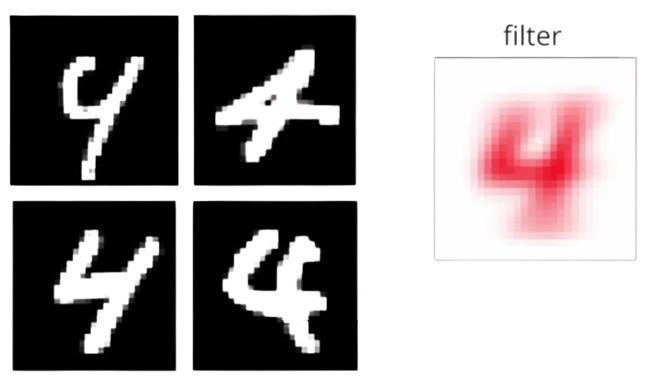
\includegraphics[scale=0.3]{3rdMTP}
\caption{Um filtro para diferentes casos.}
\end{figure}

Em alguns casos, usar apenas 1 filtro, como é feito na LR, não é o ideal. No exemplo acima, o filtro para o 4 não vai conseguir corresponder a todas as variações nas imagens. As vezes, podemos considerar situações em que temos mais de um filtro para um mesmo número:

\begin{figure}[h]
\centering
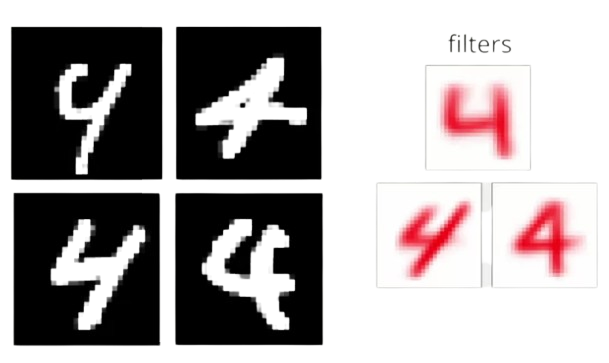
\includegraphics[scale=0.3]{4thMTP}
\caption{Multiplos filtros para vários casos.}
\end{figure}

Voltando para o \textbf{Multilayer Perceptron}:

\begin{figure}[h]
\centering
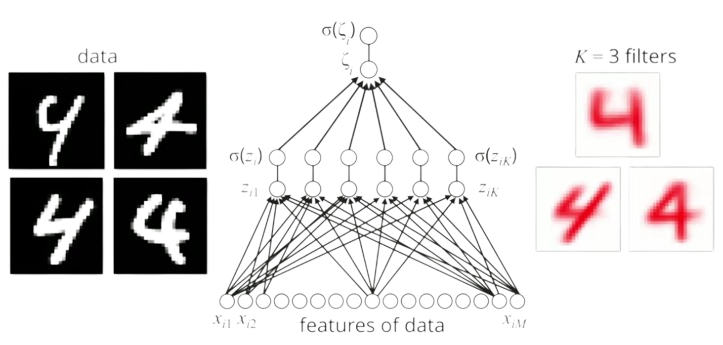
\includegraphics[scale=0.3]{5thMTP}
\caption{Multilayer Perceptron.}
\end{figure}

\subsection{Modelo Matemático para o Multilayer Perceptron}

A matemática está no coração dos modelos neurais que serão estudados. Primeiramente, é importante lembrar que o modelo estudado é uma extensão do Logistic Regression.

Nele, os dados $x_i1$ até $x_iM$ são mapeados para uma variável $z_i$ por meio do produto interno $x_i \odot b$. Isso gerava um único filtro que era aplicado a todos os dados.

A ideia do \textbf{Multilayer Perceptron} é que estamos considerando $k$ filtros e fazemos o produto interno: 

\begin{figure}[h]
\centering
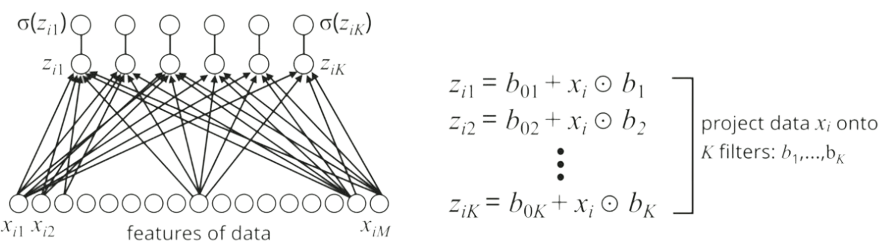
\includegraphics[scale=0.3]{6thMTP}
\caption{Como é a Multilayer Perceptron.}
\end{figure}

Então teremos $z_{i1}$ até $z_{ik}$. Esses recursos serão enviados por meio de uma Logistic Function, que é um mapeamento de um número real para um número entre 0 e 1, e fazemos isso para conseguir as probabilidade dos $k$ produtos latentes. Por fim, todos essas $k$ probabilidades latentes são enviadas por meio de um modelo de Logistic Regression para conseguir um modelo único de filtro $c$.

Assim, ao invés de conseguir o filtro $b$, passamos a ter o filtro $c$ dos dados na seguinte fórmula:
$$ \zeta _i = c_0 + \sigma (z_i) \odot c $$

Ao invés de usarmos a Logistic Regression para mapear os dados brutos para a probabilidade de um binário, passamos primeiramente por uma etapa intermediária para calcular $k$ recursos latentes que são enviados para um modelo do tipo Logistic Regression para nos dar a probabilidade de um resultado binário.

Essa adição de etapa nos permite considerar limites de decisão não lineares no espaço de recurso, como, por exemplo, o 4 escrito de diversas maneiras diferentes. Os resultados produzidos por ela se mostram mais efetivos.

\subsection{Deep Learning}

Primeiramente, vamos fazer o mesmo do anterior só que 2 vezes:

\begin{figure}[h]
\centering
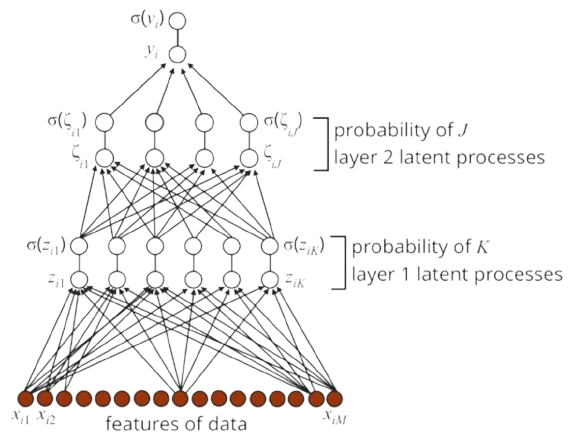
\includegraphics[scale=0.3]{7thMTP}
\caption{2 camadas de Multilayer Perceptron.}
\end{figure}

Basicamente, estamos fazendo o \textbf{Multilayer Perceptron} 2 vezes. No final de todo, ainda conseguimos uma probabilidade. O modelo é mais complicado que o anterior. Dessa forma, conseguimos entender o conceito \textit{Deep} de \textbf{Deep Learning}.

\begin{center}
\textbf{Deep Learning} é uma forma de \textbf{Machine Learning} na qual o modelo possui multiplas camadas de processos latentes.
\end{center}

Sempre, no topo, há um classificador de \textbf{Logistic Regression}, o que nos dá uma probabilidade da saída binária $Y = 1$ ou $Y = 0$.

As camadas intermediárias correspondem a $k$ recursos latentes na camada 1 e $j$ recursos latentes na camada 2. É possível ir a modelos com ainda mais camadas.

Esse clássico modelo chamado de \textbf{Multilayer Perception}, também chamado de \textbf{Neural Network}, é basicamente constituído por uma sequência de aplicações repetidas da \textbf{Logistic Regression}.
 
Cada componente do \textbf{Multilayer Perception} pode ser visto como uma aplicação repetida da \textbf{Logistic Regression}.

Porque usaríamos um modelo mais complicado?

Na \textbf{Logistic Regression}, poderíamos resolver problemas lineares, como na figura 9. Usando o \textbf{Multilayer Perception}, descobrimos que podemos aprender limites de decisão muito mais sofisticados, como na figura 10 (muitas vezes os dados estão distribuidos dessa forma).\\

Agora, um exemplo para entender sua vantagem: a análise de documentos.

\textbf{Problema:}

Um documento é um conjunto de palavras e $x_i$ representa um conjunto de features para o documento $i$. Temos um vocabulário composto de $V$ palavras e, para caracterizar um documento, simplesmente vamos contar o número de vezes que cada palavra aparece nele.

Dado o documento e as palavras que estão nele, queremos fazer uma previsão sobre se uma pessoa vai gostar ou não do documento. Like: $y_i = 1 $, dislike: $y_1 = 0$.

\begin{figure}[h]
\centering
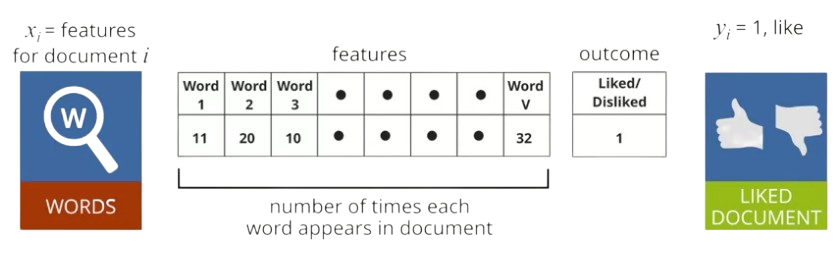
\includegraphics[scale=0.4]{8thMTP}
\caption{Exemplo documento.}
\end{figure}

Nós vamos receber dados que serão usados para ensinar o modelo, que seria o mesmo que: aprender os parâmetros do modelo.\\

\textbf{Resolução:}

Para resolver esse problema, iremos utilizar a \textbf{Multilayer Perception}.

Nesse caso dos documentos, os parâmetros $b_1, \, b_2,\, \cdots \,, b_k$ serão chamados de tópicos dos documentos. 
Podemos entender $b_1$ como palavras características de um determinado tópico, por exemplo, esportes. Portanto, dentro do vocabulário $v$, provavelmente há um subconjunto de palavras que têm alta probabilidade de aparecer no assunto esportes. Assim, esperamos que o filtro $b_1$ tenha valores altos para palavras que tenham características de esportes.

Em outro exemplo, $b_2$ pode estar relacionado com o tópico de história, com valores altos de palavras relacionadas a história e baixos caso contrário.

Uma maneira de pensar nisso é: recebemos um vetor de características $x_i$ que representa a contagem de palavras no documento. Nós vamos calcular o produto interno de $x_i$ com $k$ filtros ou templates. Eles podem ser representados como $k$ processos latentes. No contexto de documentos, podemos pensar neles como tópicos. Assim, o resultado na primeira camada diz: qual é a probabilidade desse tópico de ser sobre esportes? História? Política?

\begin{figure}[h]
\centering
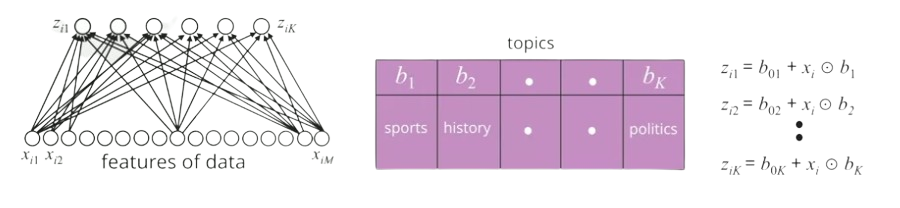
\includegraphics[scale=0.5]{9thMTP}
\caption{Análise da primeira camada.}
\end{figure}

Agora, na segunda camada, faremos a mesma coisa que na primeira: pegaremos a saída da primeira camada $z_i$, que vão passar por uma \textbf{Zigmoid Function} para transformá-lo em uma probabilidade e vamos fazer o produto interno com os filtros  $c_1, \, c_2,\, \cdots \,, c_j$ da segunda camada.

Esses filtros podem enfatizar alguns recursos da camada 1, representando meta-topics: uma combinação entre os tópicos da primeira camada. $c_1$ pode ter alto valor para os tópicos combinados de esportes e história. Se a saída de $c_1$ é grande, então o documento provavelmente é uma combinação entre os tópicos esportes e história. $c_2$ pode ser a combinação entre política e esportes, ou seja, como a política está relacionada aos esportes.

\begin{figure}[h]
\centering
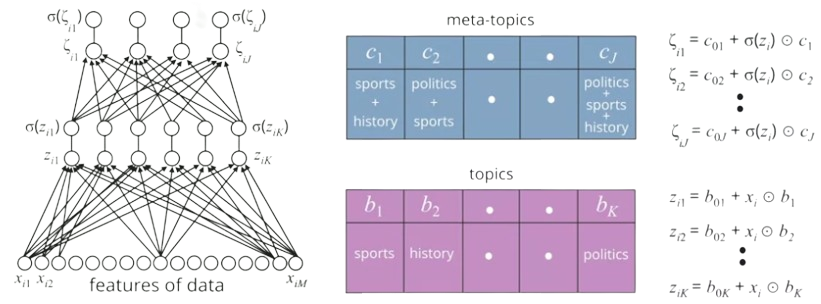
\includegraphics[scale=0.3]{10thMTP}
\caption{Análise da segunda camada.}
\end{figure}

Na primeira camada, os filtros estão procurando por tópicos; na segunda, estão buscando meta-topics: combinação desses tópicos.

Agora, na \textbf{Logistic Regression} do topo, fazemos uma pergunta: dados os meta-tópicos que parecem ser uma característica aparente dos recursos latentes na camada 2, qual é a probabilidade de a pessoa de interesse gostar ou não do documento?


\begin{figure}[h]
\centering
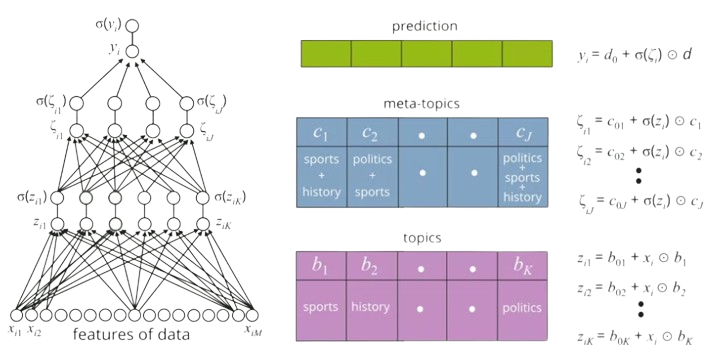
\includegraphics[scale=0.3]{11thMTP}
\caption{Análise completa com a predição.}
\end{figure}

Se uma pessoa gosta dos tópicos de esportes e história, nosso filtro $d$ procuraria a situação em que os metatópicos associados à história dos esportes é alta.

\subsection{Porque Deep Learning é tão poderoso?}

O que ele faz que não é feito facilmente por outros modelos? Usando o exemplo dos documentos: na maoria das vezes, não queremos saber se uma pessoa vai gostar de certo documento, mas sim quantas pessoas podem gostar dele. 

As 2 primeiras camadas do modelo, caracterizam o documento e não a pessoa. Consequentemente, se quisermos fazer modelos para várias pessoas, essas 2 primeiras camadas podem ser \textbf{reutilizadas} em modelos de várias pessoas. A última camada depende da pessoa.

Portanto, podemos considerar que: as camadas mais pertos dos dados possuem relação com eles e as camadas mais acima possuem relação com a pessoa. Dessa forma, posso transferir os dados de uma pessoa para a próxima quando eu já aprendi os parâmetros da parte de baixo do modelo, então só uso dados da pessoa em interesse na parte superior. Assim, temos um uso muito mais eficiente os dados.

A grande vantagem do \textbf{Deep Learning} é que podemos usar vários dados gerais de várias pessoas para construir as bases inferiores do modelo e, para analisar uma pessoa em específico, usamos o seu conjunto de parâmetros relativamente pequeno no topo.

Com a \textbf{Logistic Regression}, não podemos fazer a aprendizagem por transferência (\textbf{Transfer Learning}) da mesma forma.

\subsection{Seleção de modelo}

Há vários modelos diferentes para escolher e a melhor forma de escolher o certo é usar a experiência.

Agora, temos 2 modelos à disposição: \textbf{Logistic Regression} e \textbf{Multilayer Perceptron}.

\begin{figure}[h]
\centering
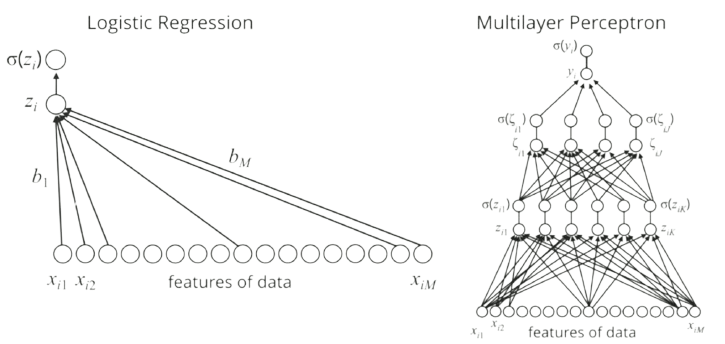
\includegraphics[scale=0.4]{12thMTP}
\caption{Um filtro para diferentes casos.}
\end{figure}

Em Machine Learning, essa escolha é chamada de \textbf{Bias Variance Trade-Off}.

O primeiro modelo, é bem simples com pouco parâmetros e o segundo é totalmente o oposto. Por isso, em cada treinamento do primeiro modelo, os resultados não terão uma grande variância, dado que é simples. No segundo, há uma maior mudança, dado a sua complexiade.

Portanto, escolhemos modelos mais simples quando não queremos muita variância. Porém essa simplicidade pode trazer uma pior performance.

\subsection{História Multilayer Perceptron/Neural Networks}

Multilayer Perceptron foi inventado por volta de 1960. Seu uso ra limitado, já que o volume de dados era pequeno e o computador não era tão potente. Em 1986, a técnica \textbf{Back Propagation} tornou a tarefa de aprender os parâmetros muito mais eficiente. Além disso, tínhamos um poder computacional bem maior. Em 1989, um modelo chamado \textbf{Convolutional Neural Network} foi desenvolvido, uma chave para análise de imagens.

No início da década de 90, os modelos foram usados em dados reais. Porém, não estavam tendo uma boa performance, pois não tinham dados o suficiente. Em 1995, surgiu a tecnologia \textbf{Long Short-Term Memory}, que era muito importante para analisar dados que variam com o tempo. O entusiasmo aumentou. 

As tecnologias que estão propulsionando o tópico hoje surgiram há relativamente bastante tempo, antes de 95, não mudaram muito.

Novamente, no início do século, a tecnologia foi para campo novamente. E a história se repetiu: não teve um desempenho tão bom.

Entre 2005 e 2010, nos principais fóruns de Machine Learning, as pessoas não falavam de Multilayer Perceptron ou Neural Networks. Estava muito mal falado.

Assim em 2010, já que isso se tornou algo bem negativo pelos seus insucessos, o nome da tecnologia foi mudado para \textbf{Deep Learning}.

Em 2013, houve uma esperança: CNN + GPU + ImageNet. Computação paralela forte, muitos dados de imagens para trabalhar. Então, a CNN foi combinada com a computação moderna, as milhares de imagens disponíveis facilmente e trouxe um avanço fundamental para seu crescimento.

Em 2015, veio o AlphaGo. Ganhar \textit{Go} contra humanos.

Durante essa história, houve vários momentos de empolgação e decepção. Nós precisamos entender quando o Deep Learning é efetivo e quando precisamos usar modelos mais simples.

\textit{"All things being equal, the simplest solution tends to be the best one."} - William of Ockham.

\pagebreak
\section{Convolutional Neural Networks}

Nessa seção, focaremos em imagens. A técnica de CNN possui um desempenho em análise de imagens maior que a dos humanos. Os dados analisados serão as imagens.

\textbf{IMG1 AQUI}

Cada imagem compõe exemplos de High-Level Motifs que são descolados para outros locais dentro da imagem. Nenhuma imagem é composta por todos os Motifs, mas cada imagem é caracterizada por um subconjunto deles e a localização deles muda em cada imagem.

As imagens na vida real possuem coisas que repetem: bordas, cantos, texturas e formatos. Isso é uma caracteristica de todas as imagens naturais. Queremos explorar isso no contexto da CNN.

a imagem geral é composta por um subconjuntos de Motifs que repetem entre as imagens.

\textbf{IMG2 AQUI}

Como podemos construir um modelo que captura essa hierarquia?

\subsection{Convolutional Example}

\textbf{IMG3 AQUI}

Nos queremos começar da parte de baixo da hierarquia e procurar por um dos elementos atômicos. Para isso, vamos mover esse triangulo em cada local da imagem. Depois, vamos calcular uma correlação que mede o quão semelhante uma região local da imagem é do nosso elemento atômico. Isso chamaremos de filtro.

\textbf{IMG4 AQUI}

Assim, ao passar esse triangulo em todos os pontos possíveis da imagem, geramos o que é chamado de \textbf{feature map}, que contém a saída do processo. O que está em vermelho mostra uma alta correlação e em azul baixa. O processo em que passamos o triângulo em toda a imagem possui um nome: convolução (convolution). Ela se manifesta ao passar o filtro (o elemento atômico) em cada local na imagem.

Nos temos múltiplos elementos atômicos, por isso iremos passar cada um desses filtros fundamentais por meio de um Two Dimensional Convolucional Process. Nós vamos conseguir um feature map para cada elemento atômico. Um mapa que reflete o grau de correspondência do elemento atômico na imagem. Portanto, conseguimos uma pilha de feature maps.

\textbf{IMG5 AQUI}

Como podemos identificar os submotifs? Vamos repetir o processo, no qual vamos convolver (convolve) filtros para cada localização bidimensional no feature map. Os filtros agora são várias pilhas de elementos atômicos.

\textbf{IMG6 AQUI}

Se um sub-motif está presente, é esperado que os respectivos feature maps associados e seus elementos atômicos tivessem uma grande amplitude próxima um do outro no espaço.

Agora, repetimos o processo: vamos fazer a convolution dos filtros da segunda camada com os feature maps da primeira. Isso vai produzir um novo conjunto de feature maps. Eles nos dirão onde cada um dos sub-motifs está na imagem. Então, repetimos esse processo novamente.

\textbf{IMG7 AQUI}

Por fim, conseguimos construir um feature map para a terceira camada.

Agora, finalmente, queremos tomar uma decisão de classficação. Ela será baseada no feature map do topo do modelo. O que é realmente importante notar sobre essa Deep Architecture é que ela se manifesta numa aplicação repetida do mesmo processo.

No início, pegamos uma imagem e a convolvemos ela com um conjunto de blocos de construção fundamentais. Depois, conseguimos um feature map, o grau de como cada um dos elementos se manisfesta na imagem. Isso nos resulta em uma pilha de feature maps.

Depois, os filtros da segunda camada procuram elementos da primeira camada que estão, simultaneamente, próximos uns dos outros. Assim, novamente convolvemos o feature map da primeira camada com os filtros da segunda, e conseguimos outra pilha de feature maps.

Por fim, pegamos os filtros dos Motifs e convolvemos com o feature map da segunda camada, o que nos gera o ultimo feature map e, com base nele, decidiremos a classificação da imagem.

No mundo real, os formatos não são tão simples quanto nesse exemplo. A pergunta é: como projetamos modelos que aprendam como construir um modelo desses para imagens reais?

\subsection{Modelo Matemático}

Tudo o que foi aprendido no exemplo ilustrado é essencialmente transferido diretamente.

Para aprender um modelo, iremos analisar milhões de imagens. O feature map reflete a intenside com que esse elemento se manifesta na imagem. Agora, vamos fazer a mesma coisa; porém, não conhecemos os elementos atômicos. Vamos representar eles por parâmetros que vamos aprender.

\textbf{IMG8 AQUI}

Em um primeiro momento, vamos assumir que sabemos os valores $\phi _1$ a $\phi_k$. Se soubermos isso, podemos construir um feature map.

$$M_n = f(I_n; \phi _1, \dots , \phi _k)$$

$M_n$ representa o feature map na camada 1 para a enésima imagem.

Então, repetimos o processo:

$$L_n = f(M_n; \psi _ 1, \dots , \psi _k)$$

Os valores $\psi _1$ a $\psi _k$ representam uma pequena pilha de imagens que querem corresponder à pilha de feature map da camada abaixo. Se eu soubesse quem são eles, eu poderia fazer a convolução. O que vamos fazer é: aprender esses parâmetros.

\textbf{IMG9 AQUI}

Podemos repetir novamente essa ideia. No topo, teremos:

$$G_n = f(L_n ; \omega _1, \dots , \omega _k)$$

\textbf{IMG10 AQUI}

Dessa forma, podemos criar um classficador que fornecerá um rótulo para essa imagem:

$$\ell (G_n; W)$$

O rótulo é uma função das features da parte superior e o parâmetros do classificador.

A diferença entre o exemplo que foi usado anteriormente é que, ao invés de  assumir as formas atômicas básicas, temos os parâmetros. O processo de filtragem convolucional é exatamente o mesmo.

O classificador poderia assumir uma forma de um Multilayer Perceptron ou um Logistic Regression. Em qualquer um dos casos, ele é caracterizado por alguns parâmetros $W$.

\subsection{Como o modelo aprende?}

\textbf{IMG11 AQUI}

A maneira com que aprendemos é supor que possuimos um acesso a um grande conjunto de dados rotulados. Uma das principais coisas que fez essa tecnologia tão poderosa foi o acesso a imensas quantidades de dados. Os dados são representados pelo par $I_n$ como a enésima imagem e $y_n$ é o rótulo da imagem.

Para simplicidade, vamos supor que os as labels são binárias, mas não precisariam ser.

No terceiro ponto, o que vamos fazer é constituir o que chamamos de uma função de energia, representado por E, que vai computar o que chamamos de de perde entre o rótulo verdadeiro $y_n$ e o do modelo, $\ell _n$.

No topo, nós conseguimos predizer o $\ell _n$ e, como estamos lidando com dados em que sabemos o rótulo, podemos calcular uma perda. Gostaríamos de fazer essa perda o menor possível.

Queremos tentar aprender ou identificar ou calcular os parâmetros $\phi$, $\psi$, $\omega$ e $W$ que minimizam essa perda. A perda é a diferença entre a precisão dos rótulos previstos e os verdadeiros.

Isso é o que queremos dizer com Machine Learning. À esquerda, está a máquina. A parte do aprendizado é pegar os dados e tentar aprender os parâmetros, de modo que a diferença entre $\ell$ e o rótulo $y_n$ seja pequena.

Porque isso é dificíl?

Um dos principais aspectos disso é que o número de parâmetros que temos que estimar é enorme, muito grande. Portanto, tentar estimá-los é difícil.

\textbf{IMG12 AQUI}

Olhando para esse gráfico, com apenas 2 parâmetros, é claro perceber que é muito difícil se mover nesse espaço para otimizar os parâmetros, pois caímos em vários máximos locais. Foi preciso de várias décadas de estudo e pesquisapara descobrir métodos de fazer isso de forma eficaz.

\subparagraph{Vantagens da Hierarquia de Features}

Se apenas os recursos do topo da arquitetura são usados para fazer a decisão de classificação, porque não podemos simplesmente criar um modelo com base nos motifs da camada superior? Qual é a vantagem dessa arquitetura profunda?

Se quisermos construir baseado apenas no topo, eles seriam aprendidos independentemente, ou seja, não saberíamos que esses filtros compartilham certas partes de sua estrutura. 

A ideia é que: ao compartilhar as estruturas os diferentes elementos dos filtros nas várias camadas, manifestada pelo fato de que todos eles são compostos de versões alteradas de blocos de construção mais fundamentais, podemos usar nossos dados de maneira mais eficiente, já que o conhecimento  de um motif pode melhorar o conhecimento de outro motif por meio da subestrutura compartilhada que eles possuem.

\begin{center}
Aprendizado é manifestado ao coletaar grandes quantidades de dados rotulados.

In general terms, the basic steps to do learning are:

Obtain a large set of labeled data

Determine the loss function, which computes loss between true label and model label

Determine parameters that minimize the sum over loss

\end{center}





\end{document}